\documentclass[11pt]{article}

\usepackage[a4paper,margin=1in]{geometry}
\usepackage{amsmath,amssymb}
\usepackage{bm}
\usepackage{booktabs}
\usepackage{siunitx}
\usepackage{microtype}
\usepackage{graphicx}
\usepackage{tikz}
\usetikzlibrary{arrows.meta,positioning,decorations.pathmorphing}
\usepackage{pgfplots}
\pgfplotsset{compat=1.16}
\usepackage[hidelinks]{hyperref}

\newcommand{\dd}{\mathrm{d}}
\newcommand{\Sc}{\mathit{Sc}}
\newcommand{\Pe}{\mathit{Pe}}
\newcommand{\Renum}{\mathit{Re}}
\newcommand{\Df}{D_{\!f}}
\newcommand{\uvec}{\bm{u}}

\title{Methodology: GPU DNS of Fractal-Interface Mixing in a Developing Duct}
\author{TorChannel --- MERGE fractal-mixing study}
\date{\today}

\begin{document}
\maketitle

\begin{abstract}
We describe the numerical methodology used to test whether a fractal
(Koch) scalar interface enhances mixing in a laminar developing pipe
flow, and how the Schmidt number $\Sc$ is swept to probe the
high-Peclet regime. The pipeline couples a GPU-accelerated, double-precision
direct numerical simulation (DNS) of the incompressible Navier--Stokes
equations --- staggered grid, fractional-step pressure projection, IMEX
time integration, Brinkman-penalized immersed pipe wall --- to a
conservative passive-scalar transport solver. To make the high-$\Sc$,
high-fractal-generation sweep tractable we exploit three physical
properties of this configuration (parallel fully-developed flow,
high-Peclet parabolicity, and an $N$-independent wall) that collapse the
cost from $O(\Pe)$ pseudo-time steps per case to a single downstream
sweep on a frozen, once-computed velocity field.
\end{abstract}

\section{Problem setup}

The configuration is a short, developing, laminar duct of square outer
cross-section $L_y \times L_z = 1 \times 1$ and streamwise length $L_x$,
inside which a circular pipe of radius $R = 0.42$ is imposed as an
immersed solid. Two co-flowing streams of a passive scalar
$c \in [0,1]$ enter the pipe at the inlet, separated by an interface.
In the \emph{baffle} configuration the dividing interface is a
\emph{Koch fractal} of generation $N$ prescribed at the inlet; the pipe
wall itself remains smooth and circular. The question is whether
increasing the interfacial generation $N$ --- which multiplies the
interfacial \emph{area} without changing the $50/50$ volume split ---
accelerates the downstream homogenisation of $c$, and how that effect
scales with the Schmidt number
\begin{equation}
  \Sc = \frac{\nu}{D}, \qquad
  \Pe = \Renum\,\Sc = \frac{U_b L}{D},
\end{equation}
where $\nu$ is the kinematic viscosity, $D$ the scalar diffusivity,
$U_b$ the bulk velocity and $L$ a reference length. The molecular
regime of interest (aqueous solutes) is $\Sc \sim 10^3$, i.e.\
$\Pe$ up to $\sim 10^4$ at the chosen $\Renum = 40$.

\begin{figure}[h]
\centering
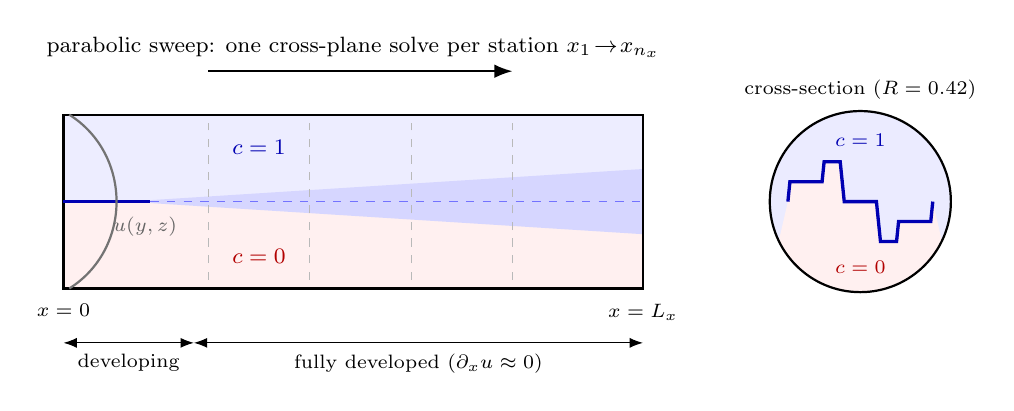
\begin{tikzpicture}[>=Latex,scale=0.92]
  % ---- main duct (side view) ----
  \begin{scope}
    \clip (0,0) rectangle (8,2.4);
    \fill[blue!7]  (0,1.2) rectangle (8,2.4);
    \fill[red!6]   (0,0)   rectangle (8,1.2);
    % mixing layer widening downstream
    \fill[blue!16] (1.2,1.18) -- (8,0.75) -- (8,1.65) -- (1.2,1.22) -- cycle;
  \end{scope}
  \draw[thick] (0,0) rectangle (8,2.4);
  % interface: sharp at inlet, diffuse downstream
  \draw[very thick,blue!70!black] (0,1.2) -- (1.2,1.2);
  \draw[blue!55,dashed] (1.2,1.2) -- (8,1.2);
  \node[blue!70!black] at (2.7,1.95){\footnotesize $c=1$};
  \node[red!70!black]  at (2.7,0.45){\footnotesize $c=0$};
  % inlet velocity profile (parabola) + flow direction
  \draw[thick,black!55] (0.08,0) .. controls (0.95,0.55) and (0.95,1.85) .. (0.08,2.4);
  \node[anchor=west,black!60] at (0.55,0.85){\scriptsize $u(y,z)$};
  % marching planes
  \foreach \x in {2,3.4,4.8,6.2} \draw[gray!55,dashed] (\x,0.12) -- (\x,2.28);
  % sweep annotation, well above the box
  \draw[->,thick] (2,3.0) -- (6.2,3.0);
  \node[anchor=south,align=center] at (4.0,3.05)
    {\footnotesize parabolic sweep: one cross-plane solve per station $x_1\!\to\!x_{n_x}$};
  % x ticks below
  \node[anchor=north] at (0,-0.08){\scriptsize $x=0$};
  \node[anchor=north] at (8,-0.08){\scriptsize $x=L_x$};
  % developing / developed bracket (own row, clear of ticks)
  \draw[<->] (0,-0.75) -- (1.8,-0.75);
  \node[anchor=north] at (0.9,-0.77){\scriptsize developing};
  \draw[<->] (1.8,-0.75) -- (8,-0.75);
  \node[anchor=north] at (4.9,-0.77){\scriptsize fully developed ($\partial_x u\approx0$)};
  % ---- cross-section inset (real N=2 Koch interface, r=3) ----
  \begin{scope}[shift={(11.0,1.2)}]
    \begin{scope}
      \clip (0,0) circle (1.25);
      \fill[blue!8] (-1.3,-1.3) rectangle (1.3,1.3);
      \fill[red!6] (-1.000,0.000) -- (-0.972,0.275) -- (-0.750,0.275) -- (-0.528,0.275)
        -- (-0.500,0.550) -- (-0.278,0.550) -- (-0.250,0.275) -- (-0.222,0.000)
        -- (0.000,0.000) -- (0.222,0.000) -- (0.250,-0.275) -- (0.278,-0.550)
        -- (0.500,-0.550) -- (0.528,-0.275) -- (0.750,-0.275) -- (0.972,-0.275)
        -- (1.000,0.000) -- (1.3,-1.3) -- (-1.3,-1.3) -- cycle;
      \draw[very thick,blue!70!black] (-1.000,0.000) -- (-0.972,0.275) -- (-0.750,0.275)
        -- (-0.528,0.275) -- (-0.500,0.550) -- (-0.278,0.550) -- (-0.250,0.275)
        -- (-0.222,0.000) -- (0.000,0.000) -- (0.222,0.000) -- (0.250,-0.275)
        -- (0.278,-0.550) -- (0.500,-0.550) -- (0.528,-0.275) -- (0.750,-0.275)
        -- (0.972,-0.275) -- (1.000,0.000);
    \end{scope}
    \draw[thick] (0,0) circle (1.25);
    \node[anchor=south] at (0,1.28){\scriptsize cross-section ($R=0.42$)};
    \node[blue!70!black] at (0,0.85){\scriptsize $c=1$};
    \node[red!70!black]  at (0,-0.9){\scriptsize $c=0$};
  \end{scope}
\end{tikzpicture}
\caption{\textbf{(Sketch, schematic.)} Configuration. Two co-flowing
scalar streams enter an immersed circular pipe separated by a Koch-folded
interface (inset, cross-section). The fully-developed velocity is frozen
and the steady scalar is obtained by a single downstream parabolic sweep.}
\label{fig:setup}
\end{figure}

\section{Governing equations}

The flow obeys the incompressible Navier--Stokes equations, with the
passive scalar advected by the resulting divergence-free velocity:
\begin{align}
  \nabla \cdot \uvec &= 0, \label{eq:cont}\\
  \frac{\partial \uvec}{\partial t} + (\uvec \cdot \nabla)\uvec
    &= -\nabla p + \nu\,\nabla^2 \uvec + \bm{f}_{\mathrm{ib}},
    \label{eq:mom}\\
  \frac{\partial c}{\partial t} + \uvec \cdot \nabla c
    &= D\,\nabla^2 c, \qquad D = \frac{\nu}{\Sc}. \label{eq:scalar}
\end{align}
All fields are stored in double precision throughout. The scalar is \emph{passive}: it does not feed back into the
momentum equation, so \eqref{eq:scalar} carries no projection step.
$\bm{f}_{\mathrm{ib}}$ is the immersed-boundary penalization force
(Section~\ref{sec:ib}). Because the conservative flux form
$\nabla\!\cdot(\uvec c)$ equals $\uvec\cdot\nabla c$ for a
divergence-free field, advection is discretised in flux form to conserve
$\langle c\rangle$ exactly.

\section{Spatial discretisation}

\paragraph{Staggered MAC grid.} Velocities live on cell faces (the
streamwise $u$ on $x$-faces, $v$ on $y$-faces, $w$ on $z$-faces) while
pressure and the scalar $c$ are cell-centred. This Marker-and-Cell
arrangement avoids odd--even pressure decoupling and gives a compact,
exactly conservative divergence/gradient pair. All fields carry a single
layer of ghost cells (indices $0$ and $-1$ in each direction) through
which boundary conditions are imposed.

\paragraph{Grid.} The mesh is uniform in the periodic-capable
$x$ and $y$ directions ($\dd x = L_x/n_x$, $\dd y = L_y/n_y$) and
\emph{stretched} in the wall-normal $z$ via a hyperbolic-tangent
mapping, clustering points near the walls; the variable spacings
$\dd z_c$ (centre-to-centre) and $\dd z_f$ (face-to-face) enter every
$z$-derivative. Spatial operators are second-order:
central differences for diffusion, and conservative flux differences for
advection. Performance-critical kernels are fused for the GPU.

\section{Time integration: fractional-step projection}

Momentum is advanced by a semi-implicit (IMEX) fractional-step
(projection) method. Within one step of size $\Delta t$:
\begin{enumerate}\itemsep2pt
\item \textbf{Explicit terms (Adams--Bashforth 2).} Advection and the
  in-plane ($x,y$) diffusion are evaluated explicitly and combined with
  second-order Adams--Bashforth,
  \begin{equation}
    \uvec^* = \uvec^n + \Delta t\!\left(
      \tfrac{3}{2}\,\bm{R}^{n} - \tfrac{1}{2}\,\bm{R}^{n-1}\right),
    \quad
    \bm{R} = \nu\nabla^2_{xy}\uvec - (\uvec\cdot\nabla)\uvec + \bm{f},
  \end{equation}
  (the first step falls back to forward Euler).
\item \textbf{Implicit wall-normal diffusion ($\theta$-method).} The
  stiff $z$-diffusion is treated implicitly,
  $\bigl(I - \theta\,\Delta t\,\nu\,\partial_{zz}\bigr)\uvec^{**}
   = \uvec^* + (1-\theta)\Delta t\,\nu\,\partial_{zz}\uvec^*$,
  with $\theta = \tfrac12$ (Crank--Nicolson). On the stretched grid this
  is a tridiagonal system per wall-normal column, solved by a batched
  Thomas solver over all columns at once. Treating only the $z$-diffusion
  implicitly removes the most restrictive viscous stability limit while
  keeping the linear solve one-dimensional.
\item \textbf{Immersed-boundary penalization} (Section~\ref{sec:ib}) is
  applied to $\uvec^{**}$ before projection.
\item \textbf{Pressure projection.} A Poisson equation enforces
  incompressibility,
  \begin{equation}
    \nabla^2 p = \frac{1}{\Delta t}\,\nabla\!\cdot\uvec^{**},
    \qquad
    \uvec^{n+1} = \uvec^{**} - \Delta t\,\nabla p,
  \end{equation}
  solved by an FFT-based fast Poisson solver in the periodic
  $x,y$ planes combined with a tridiagonal solve in $z$ (a direct
  banded solver is available as a fallback). The resulting
  $\uvec^{n+1}$ is discretely divergence-free.
\end{enumerate}

\section{Immersed pipe wall (Brinkman penalization)}
\label{sec:ib}

The circular pipe is embedded in the Cartesian box by an implicit
Brinkman (volume-penalization) force that drives the velocity to zero
inside the solid:
\begin{equation}
  \bm{f}_{\mathrm{ib}} = -\frac{\chi}{\eta}\,\uvec,
  \qquad
  \chi(\bm{x}) =
    \begin{cases} 1 & \text{solid (outside the pipe)}\\
                  0 & \text{fluid (inside the pipe)} \end{cases}
\end{equation}
with a small permeability $\eta = 10^{-4}$. The penalization is applied
implicitly to the intermediate velocity \emph{before} the projection,
$\uvec \leftarrow \uvec/(1 + \Delta t\,\chi/\eta)$, so the fast
FFT-Poisson solver is left untouched. The solid mask $\chi$ is sampled
separately on each staggered face ($\chi_u,\chi_v,\chi_w$) and at cell
centres ($\chi_c$); here it is the complement of the inscribed disc of
radius $R=0.42$ centred on the cross-section, giving a solid fraction
$\approx 0.45$. The bulk-flux controller and all mixing diagnostics are
restricted to fluid cells ($\chi_c < \tfrac12$) so that scalar diffusing
into the (non-physical) solid is never counted as mixing.

\section{Inflow / outflow boundary conditions}

The duct is open ($\mathtt{bc\_x = inout}$): periodic in $y$ only where
specified, walls otherwise, and a prescribed inlet / convective outlet in
$x$. The inlet streamwise velocity is a smooth duct profile, the product
of parabolae in $y$ and $z$ that vanish at the walls,
\begin{equation}
  u_{\mathrm{in}}(y,z) \propto
    \frac{4y(L_y - y)}{L_y^2}\,\frac{4z(L_z - z)}{L_z^2},
\end{equation}
masked to zero inside the solid and normalised so the fluid-area-mean
inlet velocity equals $U_b$. The outflow imposes zero streamwise gradient
with a global mass-flux correction enforcing
$\int u_{\mathrm{out}} = \int u_{\mathrm{in}}$ over the fluid face, so the
discrete domain conserves mass. The scalar inlet ghost is pinned to the
prescribed interface $c_{\mathrm{inlet}}(y,z)$ each step; the scalar
outflow is zero-gradient. Lateral walls use no-flux ($\partial_n c = 0$)
for the scalar.

\section{The baffle: a Koch-fractal inlet interface}
\label{sec:koch}

In the \emph{baffle} mode the pipe wall is smooth; the only $N$-dependent
ingredient is the \emph{scalar interface} prescribed at the inlet. The
two streams meet on a curve that runs wall-to-wall across the pipe and is
Koch-folded in the $y$-direction at generation $N$.

\paragraph{Generator.} The interface is built from an area-balanced
four-segment zigzag motif, each segment of length $1/r$:
\[
  (0,0)\to(\tfrac14, a)\to(\tfrac12,0)\to(\tfrac34,-a)\to(1,0),
  \qquad a = \sqrt{(1/r)^2 - (1/4)^2},
\]
valid for $1 < r < 4$. Each outward triangle is matched by an equal
inward indentation, so the fold preserves the exact $50/50$ area split at
every generation (the mean scalar is held at $\langle c\rangle = \tfrac12$).
Replacing every edge by an affine copy of the motif $N$ times yields a
generation-$N$ polyline with fractal dimension
\begin{equation}
  \Df = \frac{\log 4}{\log r}.
\end{equation}
The interfacial length (hence the area available for diffusive flux)
grows as $\sim (4/r)^{N}$ relative to the flat $N=0$ baseline, while the
enclosed area is unchanged --- isolating the effect of interfacial area
on mixing.

\begin{figure}[h]
\centering
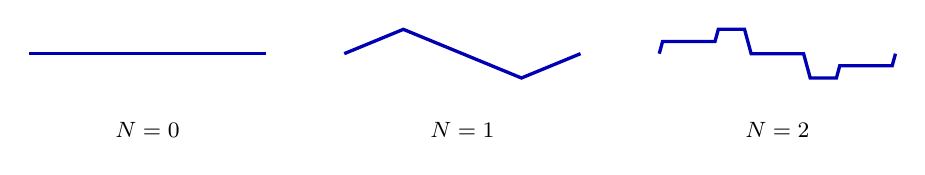
\begin{tikzpicture}[scale=1.0]
  % Real area-balanced Koch polylines (r=3).
  % N=0 flat
  \begin{scope}[shift={(0,0)}]
    \draw[very thick,blue!70!black] (0.000,0.000) -- (3.000,0.000);
    \node[anchor=north] at (1.5,-0.75){\footnotesize $N=0$};
  \end{scope}
  % N=1 (one motif)
  \begin{scope}[shift={(4.0,0)}]
    \draw[very thick,blue!70!black]
      (0.000,0.000) -- (0.750,0.309) -- (1.500,0.000) -- (2.250,-0.309) -- (3.000,0.000);
    \node[anchor=north] at (1.5,-0.75){\footnotesize $N=1$};
  \end{scope}
  % N=2 (motif applied to each N=1 edge)
  \begin{scope}[shift={(8.0,0)}]
    \draw[very thick,blue!70!black]
      (0.000,0.000) -- (0.042,0.154) -- (0.375,0.154) -- (0.708,0.154) -- (0.750,0.309)
      -- (1.083,0.309) -- (1.125,0.154) -- (1.167,0.000) -- (1.500,0.000) -- (1.833,0.000)
      -- (1.875,-0.154) -- (1.917,-0.309) -- (2.250,-0.309) -- (2.292,-0.154)
      -- (2.625,-0.154) -- (2.958,-0.154) -- (3.000,0.000);
    \node[anchor=north] at (1.5,-0.75){\footnotesize $N=2$};
  \end{scope}
\end{tikzpicture}
\caption{Area-balanced Koch generator ($r=3$, $\Df=\log4/\log3\approx1.26$).
Each edge is replaced by the four-segment motif, multiplying interfacial
length by $\sim 4/r$ per generation while preserving the $50/50$ split.
The inlet interface uses generation $N$ of this fold; these are the actual
polylines imposed.}
\label{fig:koch}
\end{figure}

\paragraph{Rasterisation.} The cross-sectional field $c(y,z)$ is set from
the signed distance $\phi$ to the open Koch polyline, smoothed over a
prescribed interface thickness $\varepsilon$ (a fixed number of cells):
\begin{equation}
  c(y,z) = \tfrac12\bigl[1 + \tanh(\phi/\varepsilon)\bigr].
\end{equation}
The distance \emph{magnitude} comes from the open polyline, but its
\emph{sign} (which stream a cell belongs to) is taken from an even--odd
point-in-polygon test against the interface closed along the far wall.
This is robust at high $N$, where a naive nearest-segment side test
produces wrong-sign corner artefacts ($N \ge 3$). The interface is
homogeneous in $x$ at the inlet; all streamwise structure that develops
downstream is produced by the flow. A companion \emph{surface\_baffle}
mode additionally folds the \emph{pipe wall} into a Koch surface,
differing from \emph{baffle} only by the wall, for a controlled
isolation of the surface-roughness effect.

\section{Passive-scalar transport}

The scalar lives at cell centres and is advanced with the same IMEX
split as the momentum equations (AB2 for advection and in-plane
diffusion; $\theta$-method for wall-normal diffusion), reusing the
batched tridiagonal solver. Advection is in conservative flux form,
\begin{equation}
  \nabla\!\cdot(\uvec c)
   = \frac{F^x_{i+\frac12}-F^x_{i-\frac12}}{\dd x}
   + \frac{F^y_{j+\frac12}-F^y_{j-\frac12}}{\dd y}
   + \frac{F^z_{k+\frac12}-F^z_{k-\frac12}}{\dd z_{f}},
\end{equation}
with face fluxes $F = U_{\mathrm{face}}\,c_{\mathrm{face}}$ built from the
MAC face velocities. Two face reconstructions are available:
\begin{itemize}\itemsep2pt
\item \textbf{Central} ($c_{\mathrm{face}}$ = linear average) ---
  second-order, used at moderate cell-Peclet.
\item \textbf{van~Leer TVD} --- a MUSCL upwind reconstruction with the van
  Leer limiter, $c_{\mathrm{face}} = c_{\mathrm{up}} +
  \tfrac12\,\psi$, monotone (no dispersive over/undershoot) at the high
  cell-Peclet of high-$\Sc$ runs. Since the face velocity is identically
  zero at every wall, the limiter never alters a wall flux.
\end{itemize}
The wall-normal boundary condition is no-flux (Neumann,
$\partial_z c = 0$), which conserves the scalar mean and lets the
segregation variance decay to zero --- the correct closure for a mixing /
decay study. A Dirichlet ($c=0$) option exists for future
sustained-gradient setups.

\section{Mixing diagnostics}

Mixing is quantified by the \emph{intensity of segregation}, the
fluid-volume-weighted, variance-based mixedness
\begin{equation}
  M = \frac{\sigma_c}{\sigma_{\max}},
  \qquad
  \sigma_c^2 = \langle (c - \bar c)^2\rangle,
  \qquad
  \sigma_{\max} = \sqrt{\bar c\,(1-\bar c)},
\end{equation}
where $\langle\cdot\rangle$ is the $z$-stretch-weighted average over
fluid cells only. $M = 1$ is fully segregated (two pure streams);
$M \to 0$ is fully mixed. For the developing duct the relevant object is
the per-slice profile $M(x)$, evaluated plane-by-plane, from which a
\emph{mixing length} $L_{\mathrm{mix}}$ is read off as the streamwise
station where $M(x)$ first falls below a threshold (e.g.\ $M = 0.9$),
linearly interpolated between planes. The fractal effect is reported as
the ratio $L_{\mathrm{mix}}(N)/L_{\mathrm{mix}}(0)$. A complementary
scalar-dissipation diagnostic $\langle|\nabla c|^2\rangle$ is also
available; unlike the gravest-mode-dominated variance, it is directly
sensitive to interfacial area and so captures the fractal's contribution
that the variance metric alone can miss.

\section{Acceleration: from $O(\Pe)$ to one sweep}
\label{sec:accel}

A direct time-march of \eqref{eq:scalar} to steady state costs $\sim\Pe$
pseudo-time steps and, at $\Sc = 10^3$ on a fine cross-section, is
infeasible. Three properties of this configuration collapse the cost.

\subsection{Parabolic space-marching (high-Peclet) scalar solver}

In a developing duct with $u > 0$ everywhere (no streamwise
recirculation), the steady scalar balance
\begin{equation}
  u\,\frac{\partial c}{\partial x}
   = D\!\left(\frac{\partial^2 c}{\partial y^2}
            + \frac{\partial^2 c}{\partial z^2}\right)
   - \left(v\,\frac{\partial c}{\partial y}
         + w\,\frac{\partial c}{\partial z}\right)
\end{equation}
is obtained after \emph{dropping the streamwise diffusion}
$\partial_{xx}c$ --- the \emph{parabolic} (boundary-layer) approximation,
asymptotically exact as $\Pe \to \infty$ and, unlike a time-march, free
of streamwise \emph{numerical} diffusion. The equation is then parabolic
in $x$ and the steady field follows from a \emph{single downstream sweep}
--- one cross-plane solve per $x$-station --- instead of marching the
unsteady field to steady state. The streamwise term uses second-order
upwind (BDF2) from the two already-solved upstream planes; each
cross-plane $(y,z)$ diffusion solve uses alternating-direction implicit
(ADI) line relaxation (a $z$-implicit then a $y$-implicit tridiagonal
sweep), which converges in a handful of inner iterations --- fastest
precisely at high $\Sc$, where the streamwise term dominates the
diagonal. Cost is $O(n_x)$ plane solves rather than $O(\Pe)$ full-field
updates. For the smooth baffle $v = w = 0$, so transverse advection is
switched off entirely.

\subsection{Frozen, fully-developed velocity (parallel-flow assumption)}

The scalar marcher runs on a \emph{frozen} velocity field. The pipe wall
is straight and $x$-independent, so the laminar flow becomes
\emph{fully developed} a short distance past the inlet: beyond the
entrance length the profile $u(y,z)$ stops changing with $x$
($\partial_x u \approx 0$) and every downstream plane is identical. We
verified this directly on the computed field --- the cross-sectional
profile is within $0.1\%$ of its developed shape by $x \approx 2.8$ and
$\partial_x u \sim 5\times10^{-5}$ thereafter. Consequently the velocity
need only be solved over the short developing region, and extending it to
an arbitrarily long scalar domain is exact: the marcher edge-clamps the
streamwise interpolation to the developed profile, i.e.\ it repeats the
one converged $u(y,z)$ downstream. This is the same parallel-flow premise
that justifies dropping $\partial_{xx}c$ in the first place; it holds
because the baffle wall does not vary with $x$ (it would \emph{not} hold
for a streamwise-varying cross-section).

\subsection{$N$-independent velocity, solved coarse and reused}

In the baffle mode the Koch generation $N$ lives only in the inlet
\emph{scalar}; the wall --- hence the entire velocity field --- is
identical for every $N$. The developed velocity is therefore solved
\emph{once} and cached, then reused across the whole $N$-sweep. Moreover
the smooth-pipe flow is well resolved on a \emph{coarse} cross-section,
whereas only the scalar needs the fine grid to resolve the Koch
striations without false diffusion. We exploit this by solving the
velocity on a coarse mesh and tri-linearly interpolating it (zeroed
inside the fine solid mask) onto the fine scalar grid. The full $N$-sweep
thus costs \emph{one} coarse velocity solve plus $N$ cheap parabolic
scalar sweeps, in place of one fine velocity solve and a high-$\Sc$
time-march \emph{per} $N$.

\section{The Schmidt-number sweep}

A sweep fixes the geometry ($R$, $L_x$, grid) and the threshold, and
varies the Koch generation $N = 0,1,2,\dots$ at a target Schmidt number.
For each $N$ the parabolic marcher returns the steady $c(x,y,z)$ on the
frozen developed velocity; from it we extract $M(x)$, the mid-plane and
cross-section slices, and $L_{\mathrm{mix}}(N)$. Comparing
$L_{\mathrm{mix}}(N)/L_{\mathrm{mix}}(0)$ across $N$, at increasing $\Sc$
(equivalently $\Pe = \Renum\,\Sc$), tests whether the fractal interface's
extra area shortens the mixing length and whether that advantage persists
into the molecular ($\Sc \sim 10^3$) regime.

\paragraph{Validation.} The scalar solver is checked against an analytic
error-function diffusion profile, exact mean conservation, and zero
numerical streamwise diffusion; the DNS divergence is monitored every
step and the run aborts if it grows.

\section{Preliminary results ($\Sc = 10$, $100$ and $1000$)}
\label{sec:results}

Table~\ref{tab:lmix} and Figure~\ref{fig:lmixN} collect the mixing length
$L_{\mathrm{mix}}$ (the station where $M(x)$ first crosses the threshold)
for the baffle, at the three Schmidt numbers run. The $\Sc=100$ and
$\Sc=1000$ data come from the parabolic marcher; the $\Sc=10$ data from a
direct time-march to steady state (an independent cross-check of the
marcher). Because $L_{\mathrm{mix}}$ grows with $\Pe$, the higher-$\Sc$
sweeps use longer domains ($L_x=6,72,90$ for $\Sc=10,100,1000$) so that
all $N$ cross $M=0.9$ within them; the threshold is therefore the
\emph{same} $M=0.9$ for every $\Sc$, an apples-to-apples comparison. The
ratio
$L_{\mathrm{mix}}(N)/L_{\mathrm{mix}}(0)$
\emph{does} depend on the threshold --- it rises smoothly toward $1$ as
$M$ is lowered (Figure~\ref{fig:thresh}) --- so every comparison here is
made at a \emph{fixed} threshold; at fixed $M$ the $N$-ordering and trend
are robust, and only the reported magnitude shifts with the choice of $M$.

\begin{table}[h]
\centering
\begin{tabular}{c
                S[table-format=1.3] S[table-format=1.3]
                S[table-format=1.3] S[table-format=1.3]
                S[table-format=2.3] S[table-format=1.3]}
\toprule
 & \multicolumn{2}{c}{$\Sc=10$ ($M{=}0.9$)}
 & \multicolumn{2}{c}{$\Sc=100$ ($M{=}0.9$)}
 & \multicolumn{2}{c}{$\Sc=1000$ ($M{=}0.9$)} \\
\cmidrule(lr){2-3}\cmidrule(lr){4-5}\cmidrule(lr){6-7}
$N$ & {$L_{\mathrm{mix}}$} & {ratio}
    & {$L_{\mathrm{mix}}$} & {ratio}
    & {$L_{\mathrm{mix}}$} & {ratio} \\
\midrule
0 & 0.492 & 1.000 & 5.490 & 1.000 & 62.818 & 1.000 \\
1 & 0.303 & 0.616 & 3.811 & 0.694 & 38.370 & 0.611 \\
2 & 0.198 & 0.402 & 2.385 & 0.434 & 26.258 & 0.418 \\
3 & 0.152 & 0.309 & 1.998 & 0.364 & 22.164 & 0.353 \\
4 & 0.136 & 0.276 & 1.936 & 0.353 & 21.657 & 0.345 \\
5 & {---} & {---}  & {---} & {---}  & 21.581 & 0.344 \\
\bottomrule
\end{tabular}
\caption{Mixing length $L_{\mathrm{mix}}$ (station where $M(x)$ crosses the
threshold) and its ratio to the flat $N=0$ baseline, baffle mode, $R=0.42$.
All at the same threshold $M=0.9$. The domain is sized so each field
decays well past the threshold: $\Sc=10$ uses $L_x=6$, $\Sc=100$ uses
$L_x=72$, $\Sc=1000$ uses $L_x=90$ (longer domains for the higher $\Pe$).}
\label{tab:lmix}
\end{table}

\begin{figure}[h]
\centering
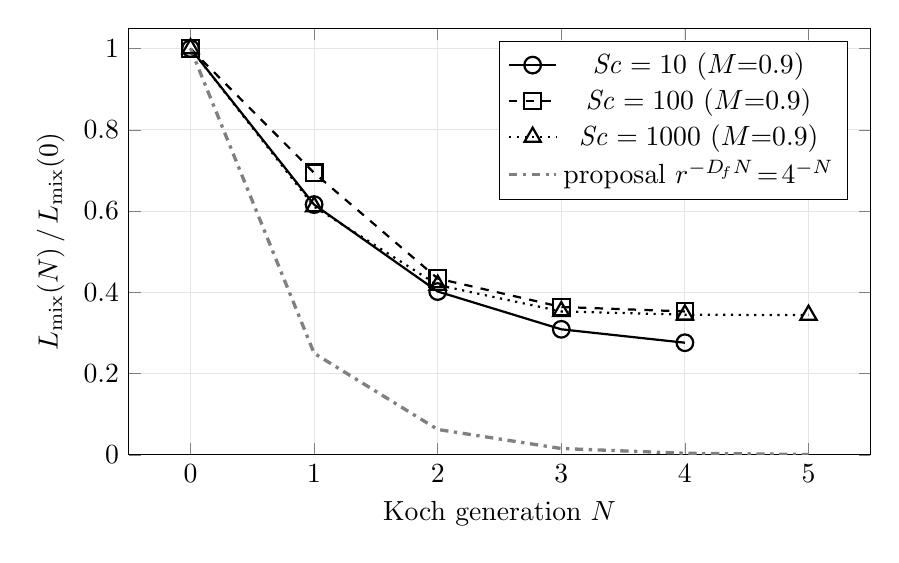
\begin{tikzpicture}
\begin{axis}[
    width=11cm, height=7cm,
    xlabel={Koch generation $N$},
    ylabel={$L_{\mathrm{mix}}(N)\,/\,L_{\mathrm{mix}}(0)$},
    xtick={0,1,2,3,4,5}, ymin=0, ymax=1.05,
    legend pos=north east, grid=both,
    grid style={gray!20},
]
\addplot[black,thick,solid,mark=o,mark size=3pt,mark options={solid}] coordinates
  {(0,1.000)(1,0.616)(2,0.402)(3,0.309)(4,0.276)};
\addplot[black,thick,dashed,mark=square,mark size=3pt,mark options={solid}] coordinates
  {(0,1.000)(1,0.694)(2,0.434)(3,0.364)(4,0.353)};
\addplot[black,thick,dotted,mark=triangle,mark size=3.4pt,mark options={solid}] coordinates
  {(0,1.000)(1,0.611)(2,0.418)(3,0.353)(4,0.345)(5,0.344)};
% proposal Eq. 4: L_mix(N)/L_mix(0) = r^{-D_f N} = 4^{-N} (r=3, D_f=log4/log3)
\addplot[gray,very thick,dash dot,mark=none,samples at={0,1,2,3,4,5}]
  {4^(-x)};
\legend{$\Sc=10$ ($M{=}0.9$), $\Sc=100$ ($M{=}0.9$), $\Sc=1000$ ($M{=}0.9$),
        proposal $r^{-\Df N}\!=\!4^{-N}$}
\end{axis}
\end{tikzpicture}
\caption{Fractal mixing enhancement, all at a fixed threshold $M=0.9$: the
mixing length falls with generation $N$ and saturates near $0.35$ by
$N\!\approx\!3$, \emph{roughly independently of $\Sc$} (the three curves
nearly overlap; $\Sc=100$ is marginally the weakest). The grey dash-dotted
line is the proposal's diffusive-limit prediction $r^{-\Df N}=4^{-N}$
(Eq.~4): the measured ratios fall well short of it --- the finite-$\Pe$
duct realises only part of the ideal exponential cut. The ratio's
magnitude depends on the threshold (Figure~\ref{fig:thresh}), but its
$N$-ordering does not.}
\label{fig:lmixN}
\end{figure}

\begin{figure}[h]
\centering
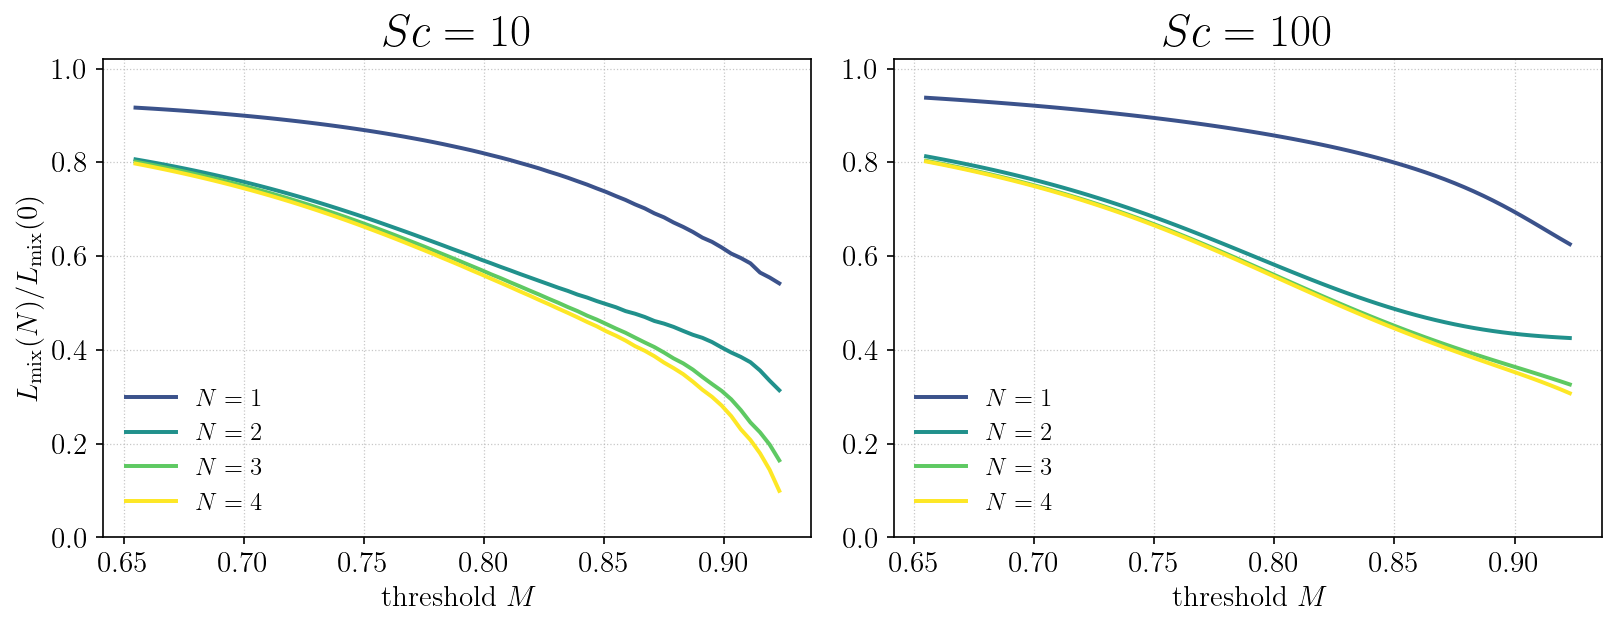
\includegraphics[width=\textwidth]{figures/baffle_ratio_vs_threshold.png}
\caption{Threshold sensitivity of the ratio
$L_{\mathrm{mix}}(N)/L_{\mathrm{mix}}(0)$: each curve is a generation $N$
(colour as in Fig.~\ref{fig:mx}) swept over the mixedness threshold $M$.
The ratio rises smoothly and \emph{monotonically} toward $1$ as $M$ is
lowered --- it never flickers or reverses --- and the $N$-ordering is
preserved at every $M$. The fractal advantage is therefore largest near
the inlet (high $M$) and fades toward complete mixing, but the qualitative
conclusions are threshold-independent; only the reported magnitude depends
on the chosen $M$. Over the same range the $\Sc=10$ and $\Sc=100$ panels
have nearly the same shape, confirming the behaviour is not $\Sc$-specific
(see also $\Sc=1000$, Fig.~\ref{fig:thresh1000}).}
\label{fig:thresh}
\end{figure}

\begin{figure}[h]
\centering
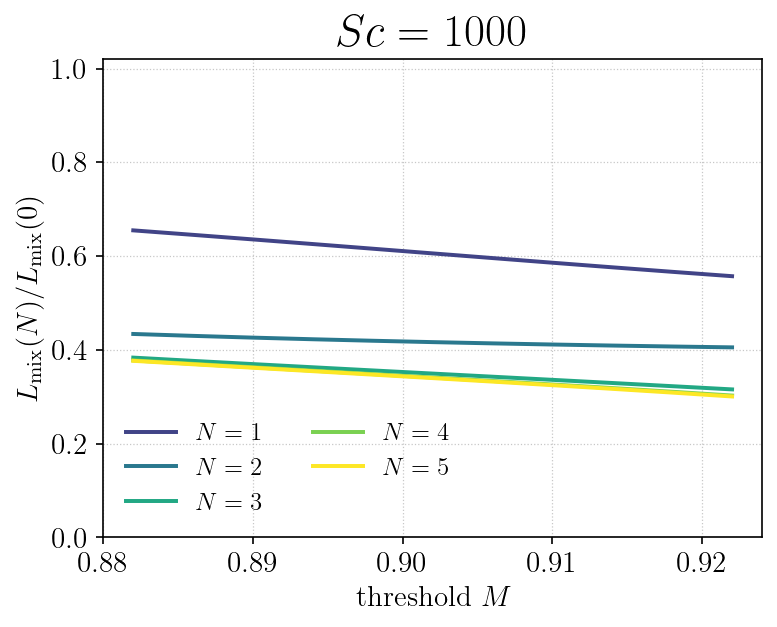
\includegraphics[width=0.55\textwidth]{figures/baffle_ratio_vs_threshold_Sc1000.png}
\caption{Threshold sensitivity at $\Sc=1000$ ($N=1$--$5$, same quantity as
Fig.~\ref{fig:thresh}). The reachable band is narrow ($M\gtrsim0.88$)
because the $L_x=90$ field mixes $N=0$ only to $M\approx0.88$; within it the
ratio is again smooth and monotone with the same $N$-ordering, consistent
with the lower-$\Sc$ panels.}
\label{fig:thresh1000}
\end{figure}

The mechanism is visible directly in the cross-sections
(Figure~\ref{fig:xsec}): higher $N$ injects more interfacial length into
the same disc, and the steep transverse scalar gradients it creates are
ground down by diffusion over a shorter streamwise distance. The
companion $M(x)$ decay (Figure~\ref{fig:mx}) shows the same ordering as a
single scalar per station, for both $\Sc=100$ and $\Sc=1000$.

\begin{figure}[p]
\centering
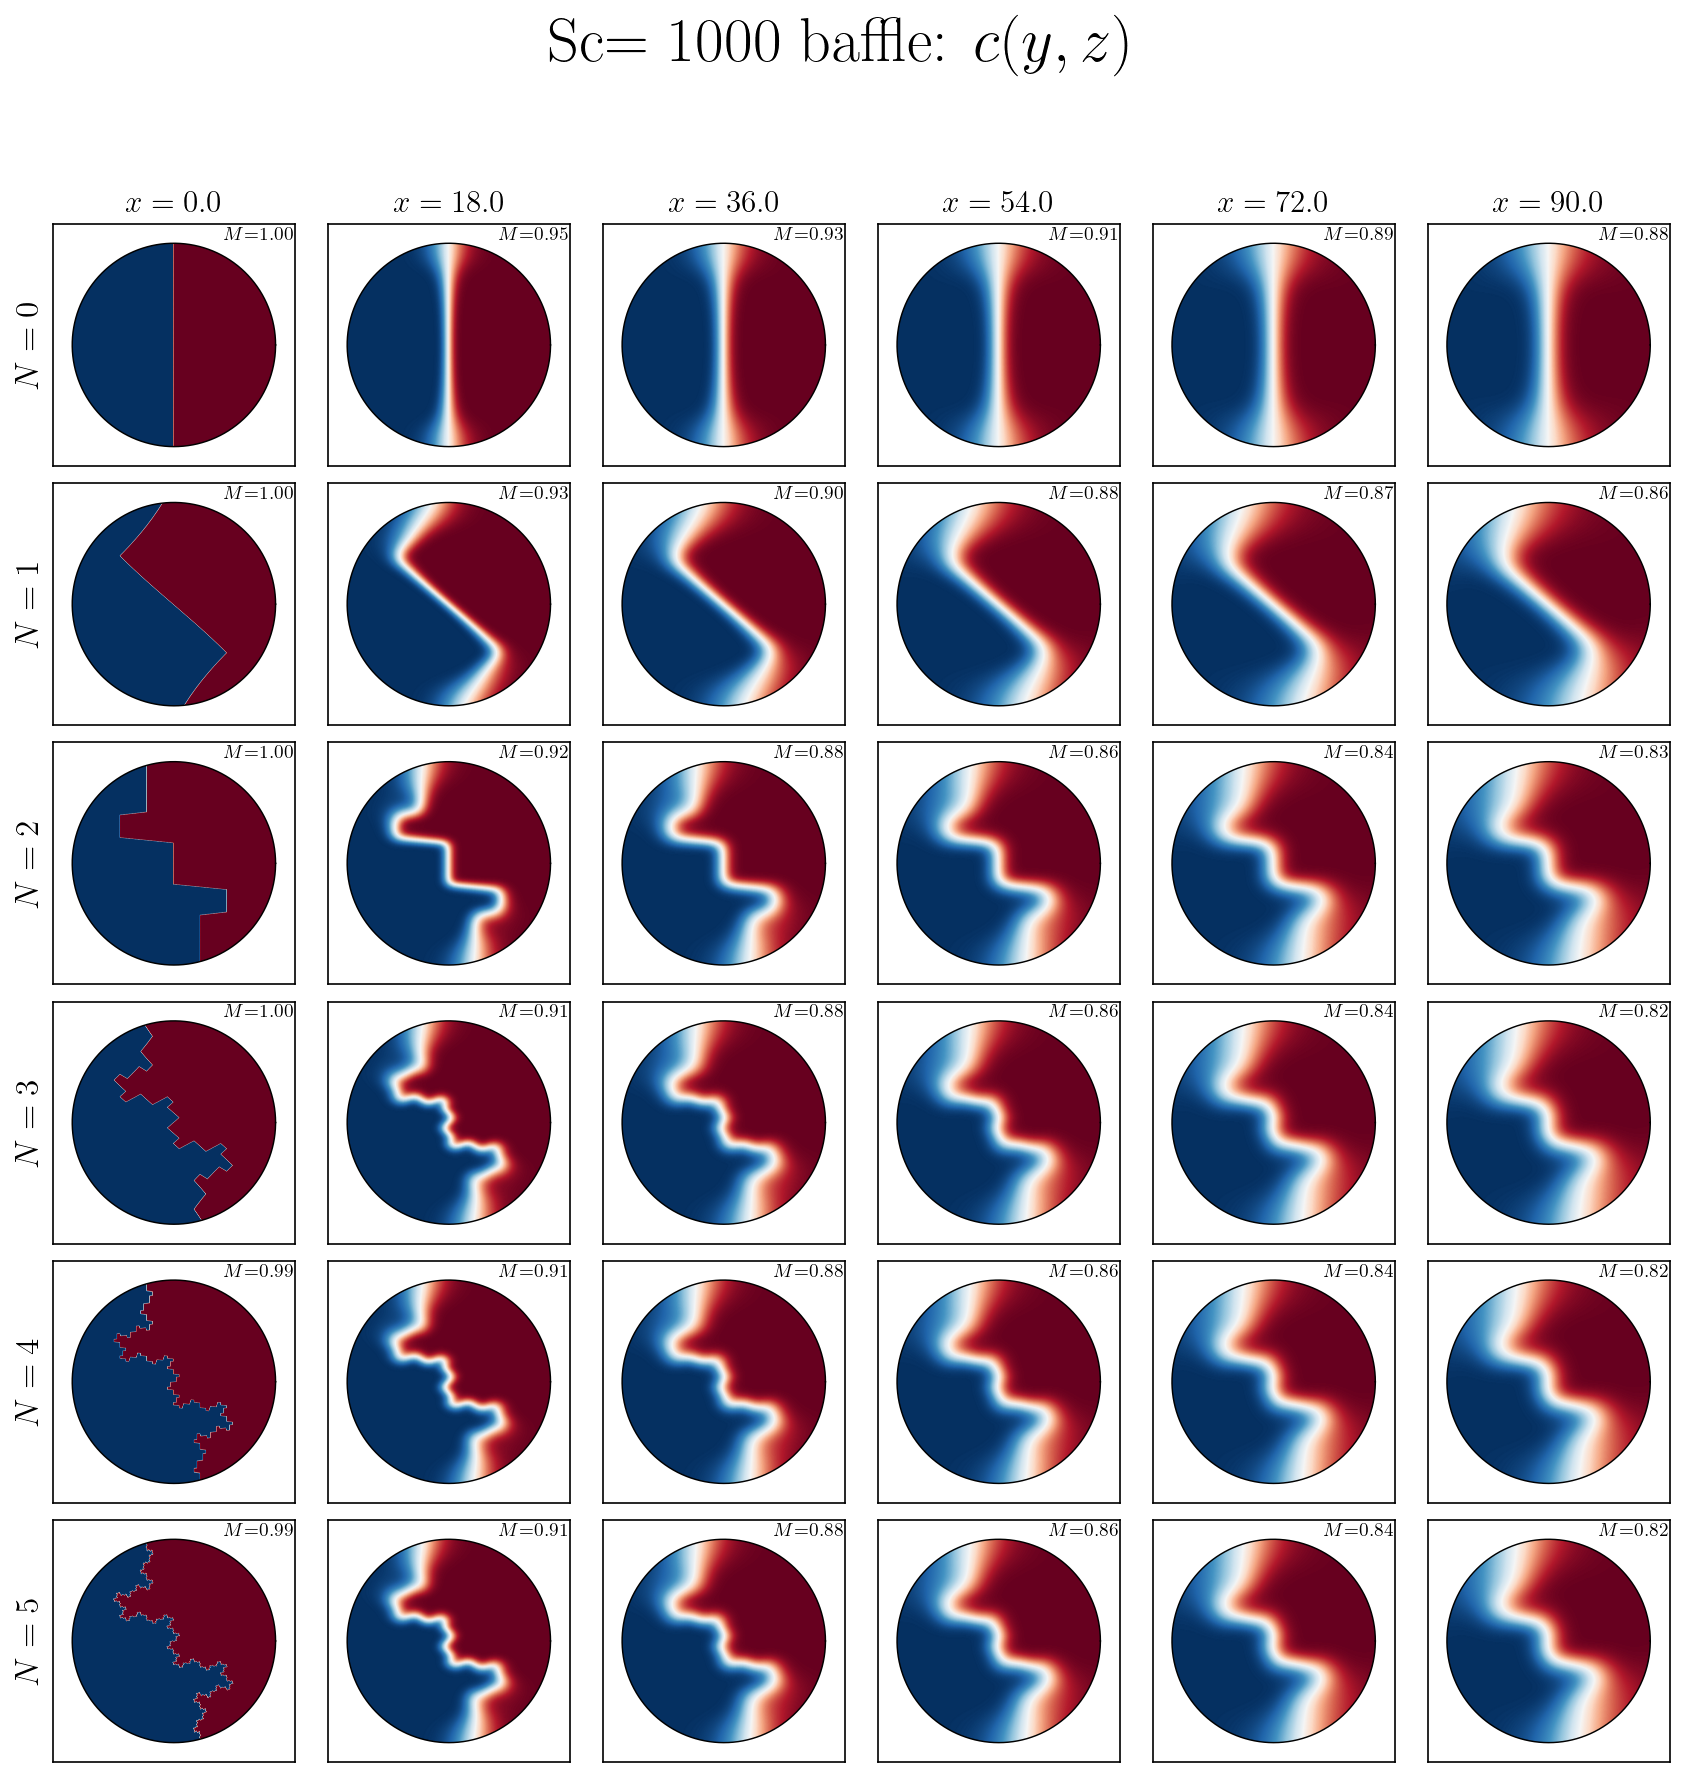
\includegraphics[width=\textwidth]{figures/baffle_Sc1000_xsections_march.png}
\caption{Steady scalar $c(y,z)$ in the pipe cross-section at $\Sc=1000$,
from the parabolic marcher. Rows: Koch generation $N=0$--$5$ (interfacial
folding increases downward). Columns: streamwise station $x=0$ (inlet)
to $x=90$ (outlet). The inlet interface ($x=0$) is the prescribed
generation-$N$ Koch fold; downstream the fractal striations diffuse and
the field homogenises faster at higher $N$ (the per-panel $M$ confirms
the trend). Same $50/50$ split and smooth wall for every $N$.}
\label{fig:xsec}
\end{figure}

\begin{figure}[p]
\centering
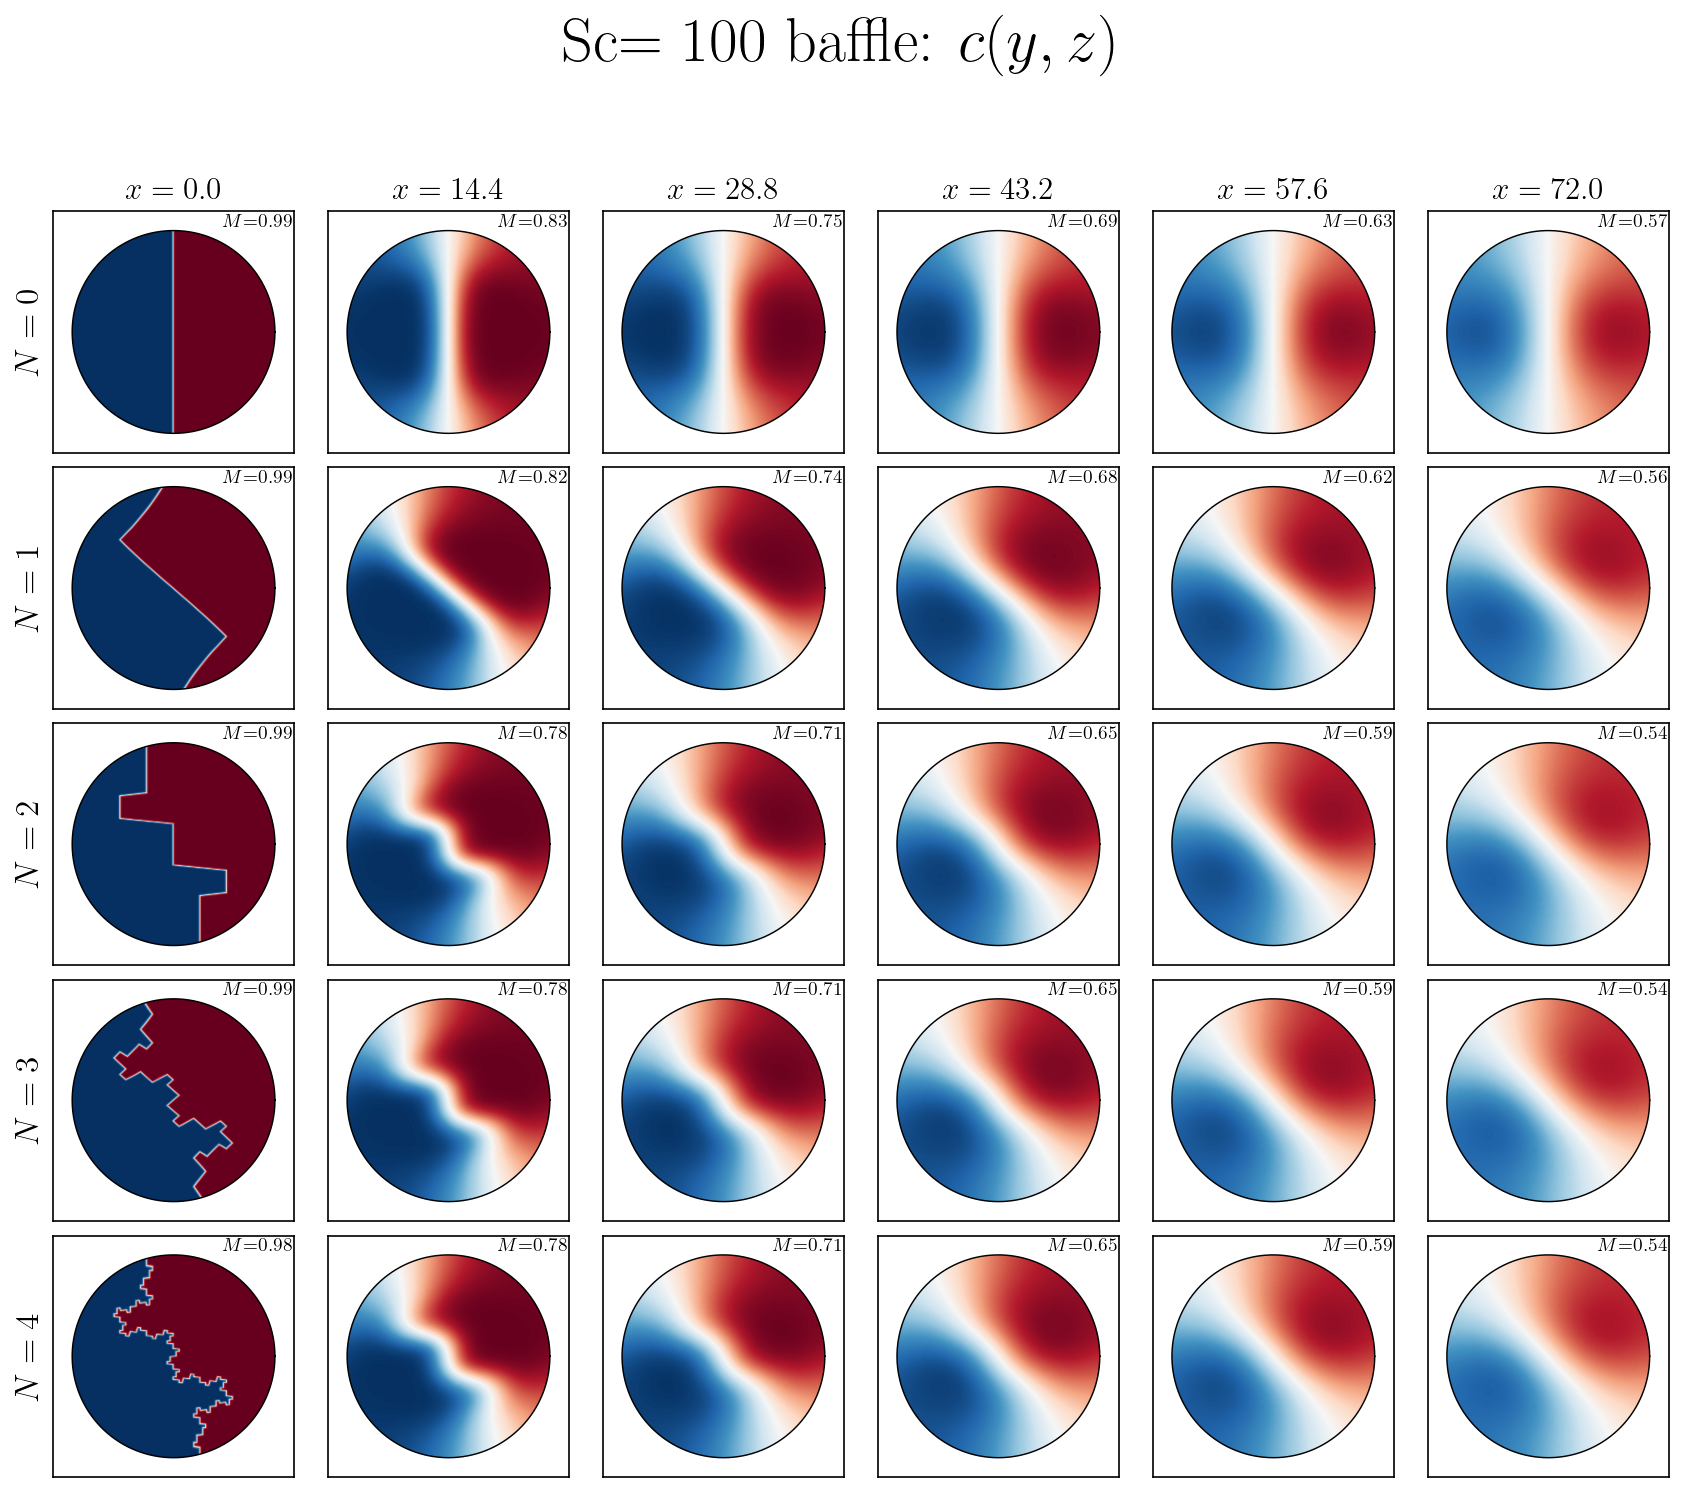
\includegraphics[width=\textwidth]{figures/baffle_Sc100_xsections_march.png}
\caption{As Fig.~\ref{fig:xsec} but at $\Sc=100$ ($N=0$--$4$, stations
$x=0$ to $72$). At the lower $\Pe$ the field mixes further within the
domain (outlet $M\!\approx\!0.54$--$0.57$); the same trend holds --- the
fractal striations diffuse out and higher $N$ homogenises sooner.}
\label{fig:xsec100}
\end{figure}

\begin{figure}[h]
\centering
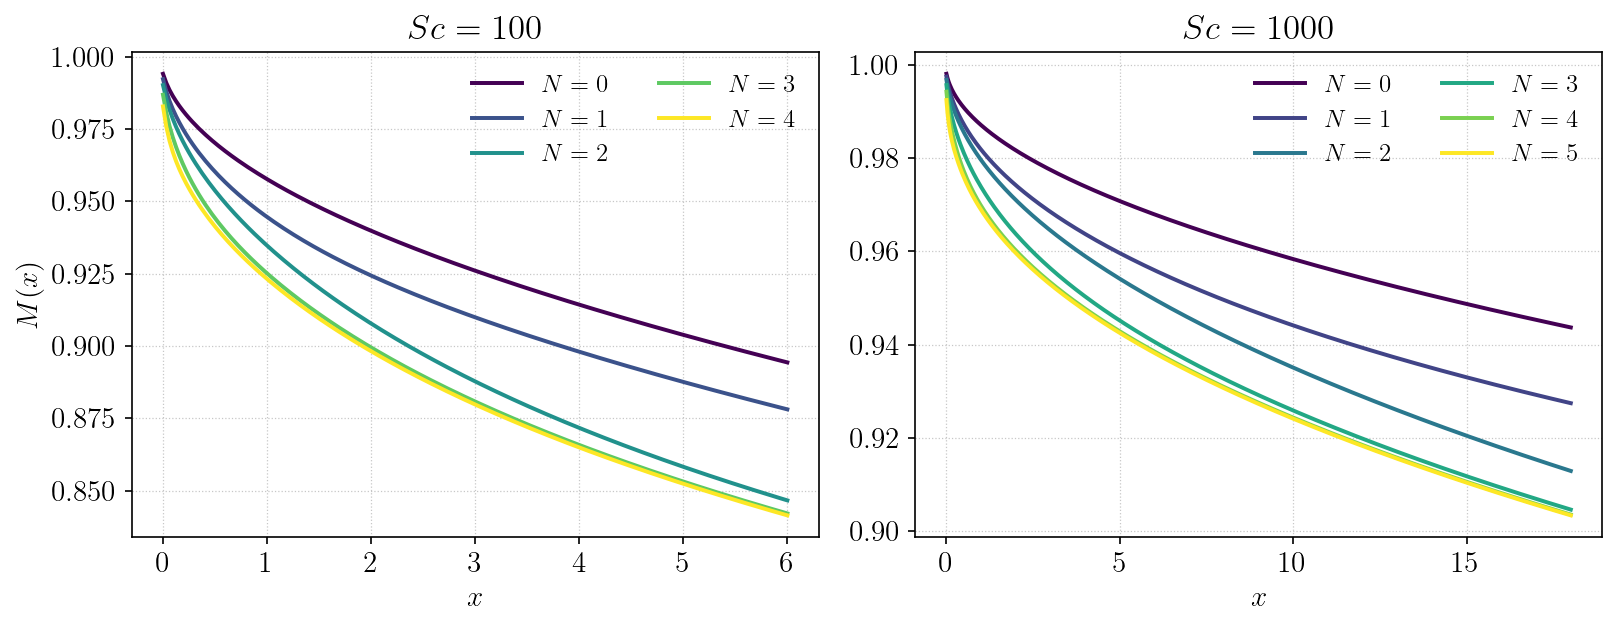
\includegraphics[width=\textwidth]{figures/baffle_Mx_double_Sc100_Sc1000.png}
\caption{Segregation decay $M(x)$, generations $N$ overlaid, for $\Sc=100$
($L_x=72$, left) and $\Sc=1000$ ($L_x=90$, right). Higher $N$ decays faster
and further in both. Both cross $M=0.9$ within their domains, so the
mixing length is read at the same threshold for every $\Sc$
(Table~\ref{tab:lmix}).}
\label{fig:mx}
\end{figure}

\section{Implications}
\label{sec:implications}

\begin{enumerate}\itemsep3pt
\item \textbf{The fractal interface robustly shortens the mixing length,
  roughly independently of $\Sc$.} At a fixed threshold ($M=0.9$), folding
  to $N=3$ cuts $L_{\mathrm{mix}}$ to $0.31$, $0.36$ and $0.35$ of the flat
  baseline at $\Sc=10$, $100$, $1000$ --- a $\sim\!3\times$ reduction that
  saturates near $0.35$ for $N\ge3$ at every $\Sc$, with the same volume
  split and the same wall. This confirms, in a resolved laminar duct, the
  core MERGE premise that interfacial \emph{area} (not bulk stirring)
  drives the enhancement. (At a \emph{common} threshold there is no clear
  monotone $\Sc$-trend --- the apparent strengthening with $\Sc$ in
  earlier mixed-threshold readings was a threshold artifact, see
  Fig.~\ref{fig:thresh}.)
\item \textbf{Diminishing returns.} Most of the gain is in the first folds
  ($N\!:0\!\to\!1\!\to\!2$); the ratio then flattens, saturating by
  $N\!\approx\!3$--$4$ at every $\Sc$ (e.g.\ $\Sc=1000$ gives
  $0.42,\,0.35,\,0.345,\,0.344$ at $N=2,3,4,5$). Folds finer than the
  local diffusion length are smeared away before they can laminate, so
  deeper fractals stop paying off.
\item \textbf{$L_{\mathrm{mix}}$ scales steeply with $\Pe$.}
  The $N=0$ baseline grows $0.49\!\to\!5.5\!\to\!63$ for
  $\Sc=10\!\to\!100\!\to\!1000$ (all at $M=0.9$) --- about a decade per
  decade of $\Sc$. This is why a high-$\Sc$ run needs a long domain, and is
  the direct motivation for the parabolic-marcher / frozen-velocity
  acceleration of Section~\ref{sec:accel}.
\item \textbf{Interfacial folding dominates over wall roughness.} The
  \emph{surface\_baffle} (Koch folds added to the pipe \emph{wall}) gives
  a weaker reduction than the interface baffle at equal $N$ (e.g.\ at
  $\Sc=10$, $N=3$: $L_{\mathrm{mix}}=0.21$ vs.\ $0.15$), indicating that
  the dominant mechanism is lamination of the scalar interface, not
  corrugation-driven secondary flow.
\item \textbf{The acceleration is what makes the proposal regime
  reachable.} Because the velocity is fully developed and $N$-independent,
  the entire multi-$N$, high-$\Sc$ sweep collapses to one coarse velocity
  solve plus cheap parabolic scalar sweeps. Without it, true $\Sc\sim10^3$
  by direct time-march would be infeasible; with it, the $\Sc=10^3$ sweep
  runs in minutes per generation.
\end{enumerate}

\paragraph{Caveats.} All ratios are quoted at a common $M=0.9$. The
$\Sc=10$ values come from a time-march on a coarse grid (some cases
stopped at the step cap, not fully steady) while $\Sc=100$ and $\Sc=1000$
use the parabolic marcher on fine grids, so cross-$\Sc$ comparisons are
indicative rather than exact --- in particular the $\Sc=10$ ratios sit
slightly below the marcher cases and should not be over-read as a trend.
The configuration and generator diagrams (Figs.~\ref{fig:setup},
\ref{fig:koch}) are schematic; the quantitative figures
(Figs.~\ref{fig:lmixN}, \ref{fig:thresh}, \ref{fig:xsec}, \ref{fig:mx})
are computed results.

\end{document}
